% !TeX spellcheck = es_ES
\chapter{Palabras nuevas}


% Intro {{{

En el capítulo anterior, se mencionó que el algoritmo toma como  idioma
dominante a aquel que transmite palabras hacia los demás y que estas perduran en los receptores al menos dos años.  El movimiento de palabras, es una característica que puede proporcionar información sobre la influencia entre los idiomas, sin embargo  puede resultar ambiguo decir que algo es más o menos influyente, además  no existe en la literatura un método que mida la influencia.

%El empleo de estás características puede proporcionar información acerca de la influencia que ejercen los idiomas,  sin  embargo, establecer un método que brinde un resultado al cual ligar la expresión influencia  no es sencillo, no existe en la literatura tal proceso, además puede ser ambiguo decir que algo es más o menos influyente sin un valor que lo respalde


%Al momento, en la literatura no existe una serie de pasos a seguir cuyo resultado final sea una cantidad que mida la influencia. Para llegar a esta resolución se requieren establecer nuevas condiciones en la base de datos, y a partir de ellas trazar posibles caminos que lleven a relaciones y resultados  con los cuales satisfacer una interpretación de la influencia

%\fxnote{ah? Otra palabra que no cuadra para nada\ldots}, 
%\fxnote{No  entiendo la ultima frase. Ten cuidado con los cambios. Siento que lo intentas hacer un poco rococo y elegante, pero por tratar, pierdes precision. Creo qeu lo mas importante  en textos cientificos es ser preciso, ordenado y conciso.}.


% \fxnote{division? No entendi\ldots}
% \fxwarning{deje comentado el texto donde me dejaste la nota y lo cmabie por el siguiente} 
% 
% \fxwarning{Ya trate de ser más conciso en lo que quiero decir, corregi todo el parrafo}
% 



 

%El llegar a esta conclusión requiere el establecer condiciones y características en los elementos para poder llegar a un resultado que satisfaga una interpretación de la influencia. 


% \fxnote{Ya no entiendo que quieres lograr con el siguietne parrafo. No se cual es el mensaje principal. De nuevo ``teñir un panorama'' no me suena correcto. Hablemos de la estructura de un parrafo y creo que tocara iterar de neuvo!!! Argh.}
% \fxwarning{ya Corregí todo el ,  dejo comentado el parrafo viejo}

%Aludiendo al capítulo  anterior, el tratamiento de la base de datos brinda información de los orígenes, los receptores y las palabras que migran de un lado a otro; comenzando con estos elementos, un primer paso es identificar los tiempos donde ocurren las migraciones. Antes de comprometer completamente al tiempo, es conveniente hacer una clasificación dentro de los propios préstamos para teñir un panorama más claro con el cual trabajar. 

Un primer paso para llegar a un valor que cuantifique a la influencia, es al estudiar los tiempos donde ocurren las migraciones, para encontrar relaciones entre dichos tiempos y las palabras involucradas en el movimiento. Antes de
profundizar en esta idea, es conveniente realizar una clasificación dentro los
préstamos, trabajar sobre ella y poder llegar a la cuantificación. 

Si se tiene una pareja de idioma origen \textit{A} e idioma receptor
\textit{B},  dentro de los préstamos de \textit{A} en \textit{B} se definen
como  \textbf{préstamos nuevos} a las  palabras que aparecen por primera vez en
las más usadas del idioma \textit{B}. Esta definición permite ordenar a los
préstamos nuevos por cada pareja de origen y receptor, y dentro  de este
ordenamiento, una segunda organización  por el año en el cual aparecieron. 



Dada la nueva clasificación, se determinaron tres posibilidades con las cuales
interpretar la influencia de un idioma sobre otro. 

\begin{enumerate}
	\label{proceso.nuevos}
	
\item Contar por cada año los préstamos nuevos de origen \textit{A} que están presentes en los diferentes receptores. Esto muestra en cuales idiomas \textit{A} ha sido influyente. 

\item Contar cuántos préstamos nuevos de diferentes orígenes están presentes en cada año, si se toma a \textit{A} como receptor. Con ello se obtienen los idiomas que han influenciado a \textit{A}

%Intercambiando a \textit{A}  como el idioma receptor, y contando cuántos préstamos nuevos de diferentes orígenes están presentes en cada año, obteniendo los idiomas que han influenciado a \textit{A}.  



\item Tomar fijos dos idiomas \textit{A} y \textit{B}, y contar cuántos préstamos nuevos de \textit{A} están en \textit{B} así como cuantos de \textit{B} lo están en \textit{A}.  Así se obtiene cómo ha sido la influencia entre \textit{A} y \textit{B}.

%contabilizando cuántos préstamos nuevos por año se encuentran al tomar a  \textit{A} como origen y a \textit{B} como receptor,  una vez hecho esto,  repetir el conteo intercambiando a \textit{B} como el origen y a \textit{A} como el receptor. Obteniendo las épocas donde alguno de ellos tuvo más del punto uno o del dos. 


\end{enumerate}


% }}}
\section{Eventos que ayudan a las migraciones} % {{{

Una parte complementaria de interpretar a la influencia es al reconocer las causas que originan las migraciones. Por ejemplo, sucesos como la globalización y el acceso al desarrollo tecnológico a finales de 1980 y principios de 1990, propiciaron la migración  de términos como \textit{internet}, \textit{computadora}, \textit{web}, \textit{email} o \textit{software}; el movimiento de este grupo de palabras se puede interpretar como una consecuencia del desarrollo e impacto de ambos eventos. 

Las causas que originan las migraciones, serán identificables a partir del significado de los préstamos involucrados en un año de migración. De acuerdo a \cite{mcgraw}, un  \textbf{campo semántico} es un conjunto de palabras asociadas que comparten parte de su significado. Entonces las palabras migrantes pueden estar relacionadas con un evento a partir de un campo semántico esto será identificable porque las migraciones ocurren en el mismo año (o en los años al rededor) donde el evento aconteció. 






%Una parte complementaria de interpretar la influencia es reconocer posibles causas que favorecen a las migraciones,  identificables por el tiempo donde ocurren, es decir, en un año de migración el significado de las palabras puede guardar alguna relación con un evento ocurrido durante el mismo año  (o en los años al rededor de él),  ya que las palabras migrantes pueden pertenecer a un mismo campo semántico relacionado al  evento. Por ejemplo, la globalización y el acceso al desarrollo tecnológico a finales de la década de 1980 y principios de 1990 propició la migración  de términos como \textit{internet}, \textit{computadora}, \textit{web}, \textit{email} o \textit{software}, mostrando a ambos ámbitos como propagadores del movimiento entre un origen y los distintos receptores. Al tratar con idiomas, se espera que en los eventos estén comprometidos países, personajes o comunidades que hablen o utilicen las lenguas involucradas. 












% }}}
\section{Préstamos nuevos entre idiomas durante el siglo XX } % {{{
\cpnote{naalisis
de palabras migrantes por pares de idiomas y tiempo, Prestamos nuevos 
por pares de idiomas}

Descritas las características que engloban a los préstamos nuevos, la obtención
y presentación de resultados se realizó de la siguiente manera. 


%Descrita la forma en que se buscarán los préstamos nuevos,  el procedimiento para la obtención y  la presentación de resultados es elssiguiente manera. 

\begin{itemize}

\item Se buscaron los préstamos nuevos entre idiomas,  durante los 109 años
comprendidos en el conjunto de búsqueda (1900-2009).
	
\item Por cada idioma, se determinó la influencia que éste ejerció en los
demás, y viceversa, mencionadas en los puntos 1 y 2
respectivamente (página ~\pageref{proceso.nuevos}).   La nomenclatura para la
cantidad de palabras nuevas será $N_{p}$.

\item Las gráficas muestran la cantidad de palabras nuevas $N_{p}$ que
aparecieron en los 109 años y a la vez, como se distribuye esta cantidad en las
diferentes décadas. 

\item Para los resultados de la influencia entre pares de idiomas (punto 3,
página ~\pageref{proceso.nuevos}), se agregó un contexto sobe las palabras que intervienen en las épocas donde hay más migraciones. Esto permite observar las áreas que influyeron en el movimiento de un grupo de palabras afín.
\cpnote{afinar}. 

\item Se proporciona en \cite{prestamos_nuevos} las listas  de préstamos nuevos
entre cada pareja de idioma origen e idioma receptor, agrupados por el año de
aparición.  Se especifica en \ref{lectura.listas}  la forma de leerlas.

\item Las palabras mencionadas carecen de signos ortográficos y su escritura es en minúsculas, ya que así provienen de la base de datos. 

%\item Los comentarios realizados, son sustentados por la influencia entre \textit{A} y \textit{B} (punto 3), las graficás correspondientes se anexan en \ref{palabras.nuevas.apendice}. 
\end{itemize}

%\fxnote{Respecto al numero en la bibliografia despues de la referencia, para que lo quieres? Creo que no es estandard y a mi me confunde. Te propongo quitarlo.}

%\fxwarning{ok, veo como quitarlo por el momento no lo se}

En las gráficas se utilizaron diferentes colores y un sistema de abreviaciones
para distinguir a los idiomas que intervienen, donde la primera abreviación
corresponde al idioma origen y la segunda al idioma receptor. Los colores y
abreviaciones se especifican  en la tabla \ref{tab.idcolor}.  En todas las
gráficas, el eje horizontal simboliza a los años del conjunto de búsqueda
(1900-2009),  mientras el eje vertical representa la cantidad de prestamos
nuevos $N_{p}$. 

\begin{table} % {{{
	\centering
	\begin{tabular}{ccc}
		\textbf{Idioma} & \textbf{Abreviación} & \textbf{Color} \\
		Inglés          & EN                   & \textcolor{C1-EN}{\rule{0.25cm}{0.25cm}}           \\
		Francés         & FR                   & \textcolor{C1-FR}{\rule{0.25cm}{0.25cm}}      \\
		Alemán          & GE                   & \textcolor{C1-GE}{\rule{0.25cm}{0.25cm}}       \\
		Italiano        & IT                   & \textcolor{C1-IT}{\rule{0.25cm}{0.25cm}}          \\
		Español         & SP                   & \textcolor{C1-SP}{\rule{0.25cm}{0.25cm}}        
	\end{tabular}
	\caption{Nomenclatura de los idiomas.}
	\label{tab.idcolor}
\end{table} % }}}

\begin{figure} % {{{
	\centering
	\begin{tabular}{cc}
		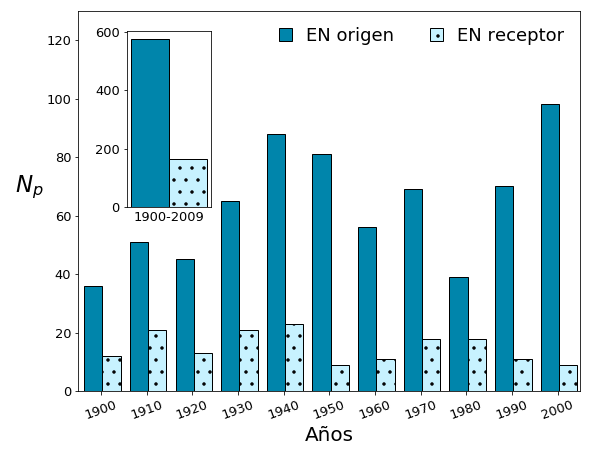
\includegraphics[width=0.5\textwidth]{BOR_EN.png} &
		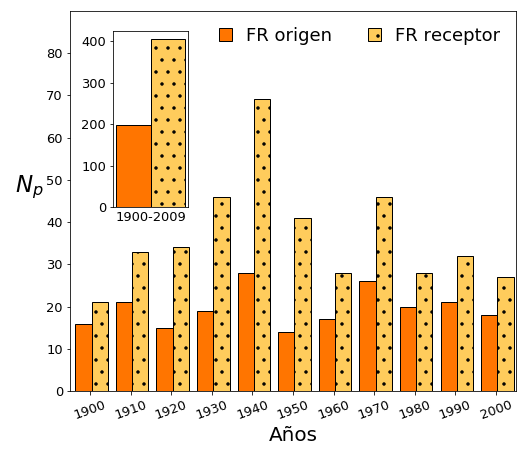
\includegraphics[width=0.5\textwidth]{BOR_FR.png} \\
		\textbf{(a)} & \textbf{(b)}   \\
	\end{tabular}

	\begin{tabular}{cc}
		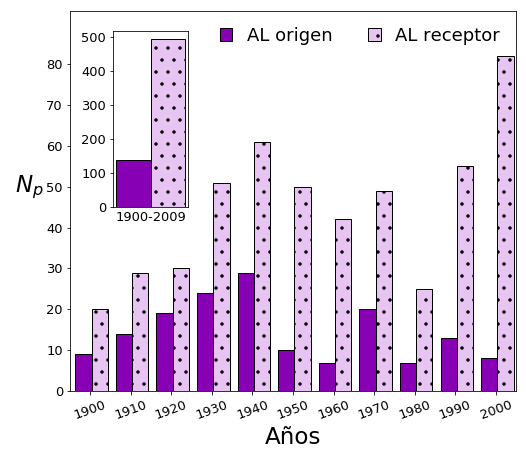
\includegraphics[width=.5\textwidth]{BOR_GE.png} &
		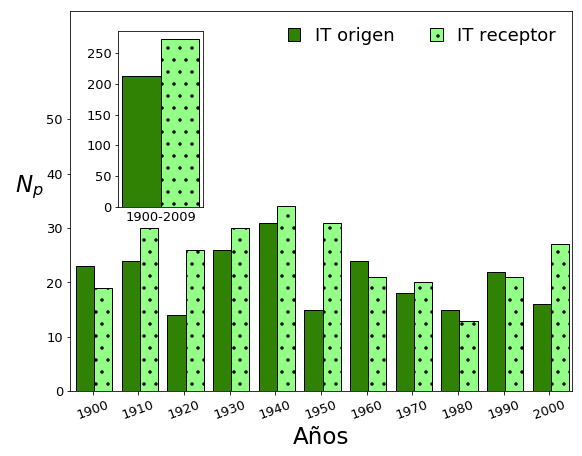
\includegraphics[width=.5\textwidth]{BOR_IT.png} \\
		\textbf{(c)}  & \textbf{(d)}   \\
	\end{tabular}
	\begin{tabular}{c}
		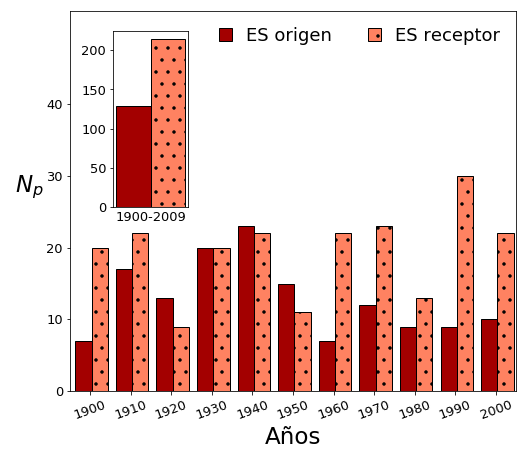
\includegraphics[width=.5\textwidth]{BOR_SP.png} \\
		\textbf{(e)} \\
	\end{tabular}
	\caption{Los idiomas como orígenes y receptores de palabras nuevas.
	Durante el siglo XX, sólo el inglés \textbf{(a)} ha sido el idioma que
	ha aportado más palabras de las que ha recibido. Francés \textbf{(b)},
	alemán \textbf{(c)}, italiano \textbf{(d)} y español \textbf{(e)}, han
	recibido más palabras durante la segunda mitad de siglo, tras finalizar
	la segunda guerra mundial. }
	\label{fig.RO_idiomas}
\end{figure} % }}}

La figura~\ref{fig.RO_idiomas} muestra el comportamiento de los idiomas al ser
orígenes o receptores de palabras nuevas.  El inglés ha aportado casi tres
veces más palabras de las que ha recibido, con sus mayores apogeos en 1940,
década que aconteció la segunda guerra mundial,  y en el 2000 tras la
globalización y el acceso a la tecnología en mayores sectores de la población. 

Francés y alemán, como receptores han sido similares, ambos recibiendo casi la
misma cantidad de palabras en cada década desde comienzos (1900) hasta mitad de
siglo (1950). Después de 1980, el alemán ha obtenido en cada década 30 palabras nuevas respecto a la década anterior, en consecuencia ha sido el mayor receptor en los últimos treinta años. Al tratarse como idioma origen, el alemán redujo la cantidad de palabras que aportaba en 1950, nuevamente tras finalizar la segunda guerra.

Referente al italiano, década a década, aporta casi la misma cantidad de
palabras que las que recibe, las únicas excepciones se dieron en 1920 y en
1950, tras finalizar la primera y segunda guerra mundial. 

Finalmente, el español en 1930 y en 1940, la cantidad de palabras que aporta y
que recibe es similar.  En las demás épocas, el español ha actuado primordial
mente como un idioma receptor. 

\subsection{Inglés} % {{{
\cpnote{aca vamos en el 3}

\begin{figure} [h!] % {{{
	\centering
	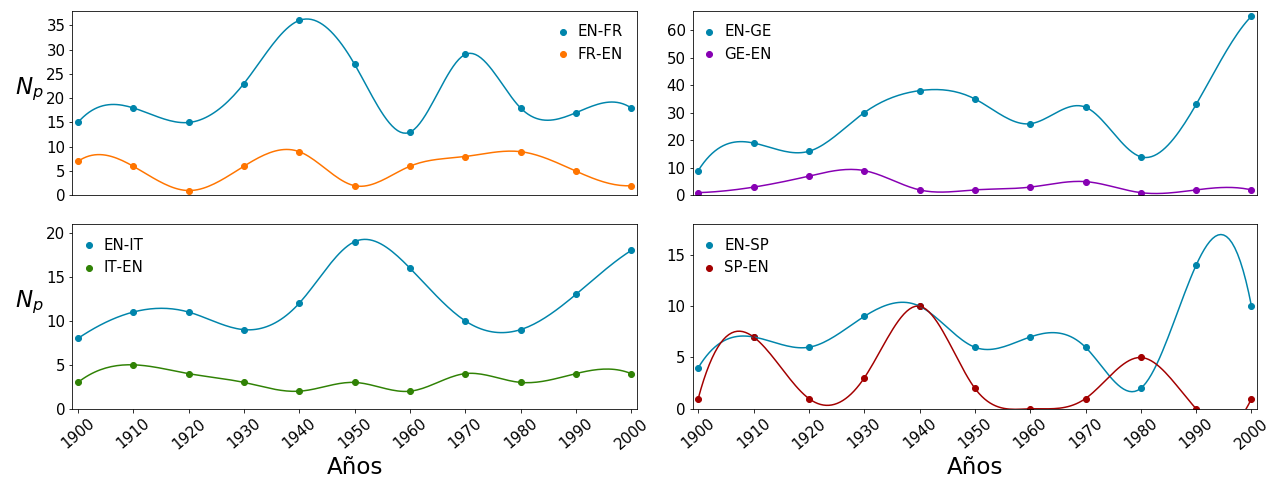
\includegraphics[scale=.33]{NC_EN.png}
	\caption{Palabras nuevas del inglés en los demás idiomas. El alemán se ha beneficiado más del inglés, con los mayores aportes en los primeros años del siglo XXI. Las características de palabras que aporta el inglés son términos políticos, industriales y del desarrollo tecnológico.}
	\label{fig.NC_EN}
\end{figure} %  }}}

%De manera general, el idioma que más se ha beneficiado del inglés ha sido el alemán, con 300 préstamos en 100 años.  Inglés y alemán forman parte de las lenguas germánicas,  posible razón de los mayores intercambios. Entre las lenguas romances, el francés fue el más favorecido, pero también es la más similar por las relación normanda entre ambas.

A partir de la figura~\ref{fig.NC_EN}, es apreciable que el inglés
ha sido el mayor portador de palabras nuevas en cualquier combinación, salvo en los periodos de 1910, 1940 y 1950,  donde recibió del español tantas palabras nuevas como las que aportó.

A pesar de ser el mayor portador, la cantidad de palabras nuevas en los diferentes receptores no es homogénea, por ejemplo en el francés  la cantidad mínima por década es de 13, mientras que el español recibió un máximo de 14 en 1990.  Al tomarse como receptor hay más homogeneidad, ya que la media de palabras recibidas por década en cualquier combinación ronda  entre 3 y 5. 

Entre 1920 y 1950, los receptores francés, alemán  e italiano, tuvieron un incremento de palabras del inglés; en este periodo se suscitaron las dos guerras mundiales, donde países de las cuatro lenguas estuvieron involucrados, a diferencia del español con una participación mínima en ambos conflictos y donde el incremento apenas fue perceptible.   

Una tendencia similar se dio en los últimos veinte años (1980-2000), con un incremento en el alemán, el italiano y el español; el hecho al que se relaciona tal incremento es que el inglés se ha mostrado como un idioma común en la comunicación, la ciencia y la tecnología,   sumado al poder que obtuvo los Estados Unidos tras la segunda guerra mundial y donde su modelo económico prevaleció después de la guerra fría (conflicto que termino en 1990). 



\subsubsection*{Inglés-Francés} % {{{


Los mayores aportes se dieron entre 1930 y 1970, periodo que engloba comienzos de la gran depresión (1929), la segunda guerra mundial (1939-1945) y la guerra fría (1945-1991), sucesos donde participaron países de ambas lenguas. Las palabras nuevas que refieren a estos eventos son \textit{churchill} (1944), \textit{territories} (1944), \textit{nazis} (1945), \textit{catastrophe} (1945), \textit{dollar} (1950), \textit{nixon} (1968) y \textit{johnson} (1970); las ultimas son apellidos de los presidentes de los Estados Unidos  Lyndon B. Johnson y Richard Nixon, cuyos periodos de gobierno fueron  entre 1963-1969 y 1969-1974 respectivamente.

% }}}
\subsubsection*{Inglés-Alemán} % {{{

Sólo  en dos épocas (1900  y 1980), el alemán no fue el idioma que más prestamos recibió  del ingles. Por el año de aparición, palabras como \textit{economic} (1929), \textit{depression} (1931), \textit{investment} (1933) y \textit{roosevelt} (1935), son del campo semántico de la economia y de la gran depresión,  mientras que  Franklin D. Roosevelt fue el presidente de los Estados Unidos que gobernó posterior a la crisis económica y durante la segunda guerra mundial. 

%La crisis económica de la gran depresión, originada en los Estados Unidos con consecuencias en diferentes países, entre ellos  Alemania, fue uno de los motivos que propició la segunda guerra mundial.

En las ultimas dos décadas, surgen términos referentes a la globalización y al desarrollo tecnológico, entre ellas \textit{standards} (1983), \textit{market} (1994), \textit{internet} (1996), \textit{economy} (1996), \textit{online} (1998), \textit{value} (2001), \textit{financial} (2003) y \textit{customer} (2007). 
% }}}

\subsubsection*{Inglés-Italiano} % {{{


Las palabras hacia el italiano, identificables en la primera mitad de siglo son \textit{roosevelt} (1941) y \textit{stalin} (1949), apellidos de personajes involucrados en la segunda guerra mundial. En el caso de Joseph Stalin, a pesar de que su nacionalidad no es de algún país de habla inglesa, en el inglés su apellido tomó notoriedad para exportarse a los otros idiomas, siendo un ejemplo de palabras que se hacen populares en idiomas distintos al idioma origen. 

En los últimos años, nuevamente la globalización y la economía, son áreas comunes para los préstamos del inglés, \textit{internet} (1996), \textit{bussines} (2000) y \textit{marketing} (2001), son ejemplos de ellas. 


\subsubsection*{Inglés-Español} 

% aclarar esta justificacion
El español ha sido en cada década  el idioma que menos prestamos toma del ingles, sin embargo las relaciones encontradas han sido las más bastas.  Nombres de organizaciones y empresas,  \textit{standard} (1933) (referentes a la extinta Standard Oil, migrando \textit{oil} (1931) dos años antes) y \textit{unesco} (1955);  presidentes de los Estados Unidos,  \textit{roosevelt} (1941), \textit{kennedy} (1961), \textit{johnson} 1966),  \textit{nixon} (1972) y \textit{bush} (1990); y la globalizacion, \textit{internet} (196), \textit{mail} (1999), \textit{marketing} (2001) y \textit{software} (2004).   

%A pesar de no ser el idioma más favorecido es al que en más areas ha impregnado el ingles, siendo este un factor que también puede indicar una mayor influencia,  en cuantas áreas esta presente un idioma y que tanto se utiliza. 

% }}}
% }}}
\subsection{Francés} % {{{

\begin{figure}[h!]
	\centering
	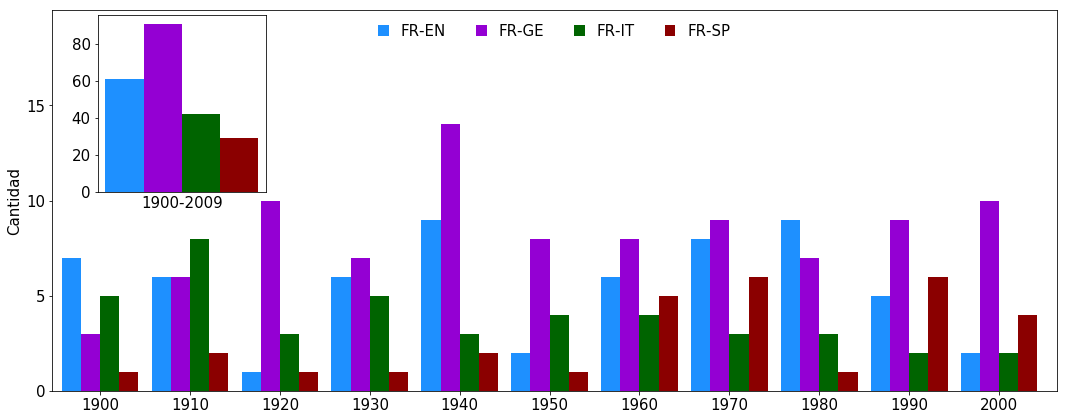
\includegraphics[scale=.33]{NC_FR.png}
	\caption{Palabras nuevas del francés en los demás idiomas. Entre las lenguas romances, el aporte del francés ha sido minoritario, mientras que en las lenguas germánicas el francés llevó más elementos, principalmente en el alemán, durante la primera (1920) y segunda guerra mundial (1940).}
	\label{fig.NC_FR}
	
	
\end{figure}

La figura~\ref{fig.NC_FR} muestra al francés como un idioma variante en cuanto a ser mayormente portador o receptor de palabras nuevas. En el inglés y el italiano, actuó principalmente como receptor,   en ambos idiomas,  el francés adoptó más palabras en la década de 1940,  nuevamente surge como factor común de las migraciones la segunda guerra mundial.

El francés con el alemán y el español tiene un comportamiento similar en algunos periodos; del alemán adoptó tantas palabras como dio (salvo en 1930 tras la gran depresión) hasta 1940, posteriormente existió una diferencia promedio de tres palabras entre las dadas y las adoptadas. En el español hasta 1940, hubo una palabra de diferencia entre las recibidas y las otorgadas. De estas características, se puede decir que el comportamiento del francés al ser origen de nuevas palabras fue (casi) de la misma forma que al ser receptor, con el alemán durante todo el siglo, y con el español en la primera mitad. 




\subsubsection*{Francés-Inglés}% {{{

Durante el siglo XX, los préstamos en este sentido, se caracterizan por ser palabras comunes e identificables de origen inglés,  por ejemplo  \textit{diagnostic,} \textit{clients,} \textit{placement,} \textit{adaptation,} \textit{diffusion,} \textit{amplitude,}.  A pesar de ser errores en los resultados, este tipo de palabras si surgieron primero en el francés, por lo que el algoritmo designó a esta lengua como el origen. 

% }}}
\subsubsection*{Francés-Alemán}% {{{

El alemán tuvo dos décadas entre 1920 y 1940  (años cercanos a las dos guerras mundiales), donde  fue el idioma que más palabras adopto del francés, , se ubicaron a  textit{diplomatie} (1917), \textit{bourgeoisie} (1919),  \textit{guerre} (1925), \textit{allemagne} (1925), \textit{russie} (1925) y \textit{empire} (1937); palabras del campo semántico de la politica, y que es acorde a ambas contiendas. 


% }}}
\subsubsection*{Francés-Italiano}% {{{

Las clasificaciones para esta pareja de origen y receptor son escasas, entre las pocas realizadas se encuentra un término del campo científico como \textit{poincare} (1924) (apellido del matemático francés Henri Poincaré);  y nombres de ciudades y países referentes tras las dos guerras mundiales, \textit{versailles} (1924), \textit{vietnam} (1966)  y \textit{urss} (1975).


% }}}
\subsubsection*{Francés-Español}% {{{

Al igual que en italiano, en  español hay pocas palabras cuyo contenido fue ligado a un evento. La palabra más destacada es \textit{euros} (2002),
nombre y primer año de circulación de la moneda de la unión europea, organización donde son miembros España y Francia. 

%El hecho de no poder enlazar palabras a eventos, no significa que el francés no es importante para el español (o el italiano), sino que el periodo donde los hechos tuvieron mayor impacto no esta dentro del periodo de búsqueda,  por ejemplo hechos como la revolución francesa, o la invasión napoleónica a España, propiciaron a un mayor intercambio en este sentido, pero al ocurrir antes de 1900 no permite tener una conclusión de ello. 


% }}}
% }}}
\subsection{Alemán}% {{{

\begin{figure}[h!]
	\centering
	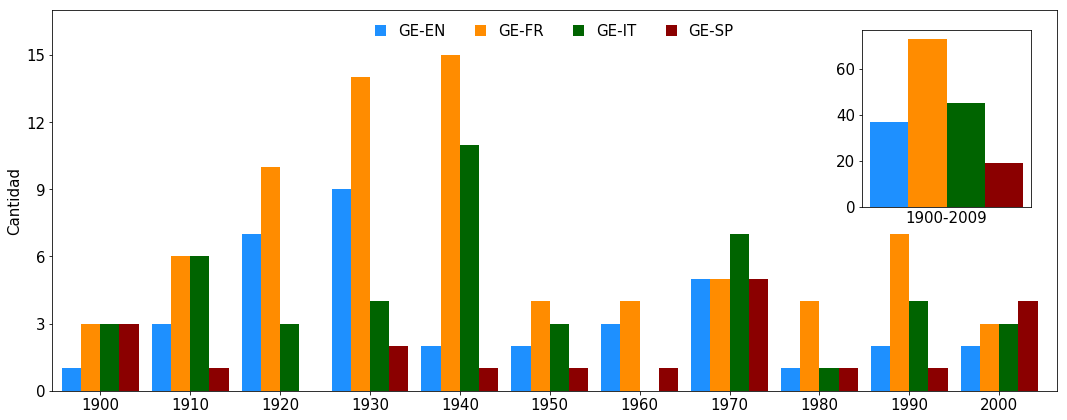
\includegraphics[scale=.33]{NC_GE.png}
	\caption{Palabras nuevas del alemán en los demás idiomas. El francés destaca  entre 1930-1940 por ser el idiomacordes a ambas contiendas con más préstamos del alemán. Se distingue al español por tener periodos donde no recibió alguna palabra.}  
	\label{fig.NC_GE}
\end{figure}


De acuerdo a la figura~\ref{fig.NC_GE} el alemán ha sido el idioma que menos préstamos aportó , en el francés en cada década hubo al menos tres  palabras, mientras que en los demás existieron años donde el aporte fue nulo, 1900 y 1980 en el ingles,  1960 en el italiano y 1920 en el español. Como portador de palabras, todos los receptores obtuvieron palabras del alemán entre 1930 y 1940, sin embargo después de esta época se dan los periodos antes mencionados donde el aporte es nulo. 

La participación del alemán en los conflictos bélicos del siglo pasado pudo ser un factor para que el alemán actuara más como un idioma receptor, adaptándose a ámbitos culturales, políticos y económicos, reflejando en periodos comunes en las migraciones, entre 1910 y 1920 (primera guerra mundial) todos los idiomas crecieron en el alemán,  durante 1940 y 1970  (fin de la segunda guerra mundial y apogeo de la guerra fría) las migraciones fueron estables, y finalmente  se dio un segundo periodo de crecimiento entre 1980 y el 2000 (fin de la guerra fria y unificación de Alemania). 





\subsubsection*{Alemán-Inglés}% {{{

En los años posteriores a la segunda guerra mundial, se encontraron palabras ligadas al evento, entre ellas \textit{lenin} (1931), \textit{hitler} (1934) y \textit{reich} (1939).  Otras palabras relevantes son \textit{beethoven} (1930), \textit{marx} (1934) y \textit{freud} (1934), apellidos de personajes destacados en la música, la filosofía y la psicología. 


% }}}
\subsubsection*{Alemán-Francés}% {{{

%El francés ha recibido más palabras del alemán que cualquier otro. A pesar de que la mayor cantidad de aportes se dio en la primera mitad de siglo, las relaciones que se encontraron han sido a lo largo de todo el periodo y en diferentes áreas. 

Se distinguieron dos campos comunes para los préstamos nuevos,  el primero referente a la  la historia del alemán en las guerras, \textit{kaiser} (1915), \textit{reich} (1921), \textit{hitler} (1933),  \textit{regierung}, \textit{deutschen},\textit{minister} y  \textit{bestimmungen} (traducciones de gobierno, alemán, ministro y reglamentos) las ultimas surgieron en 1944.  

El segundo campo, son apellidos de  personajes destacados en la historia, la filosofía, la música y la psicología, además de Hitler, se encuentra  \textit{nietzsche} (1905),  \textit{marx} (1923),  \textit{mozart} (1956), \textit{freud} (1965), \textit{engels} (1970) y \textit{heidegger} (1987); todos ellos  nacidos en países germanohablantes.

% }}}
\subsubsection*{Alemán-Italiano}% {{{

Nuevamente los préstamos que aporta el alemán,  son apellidos de personajes,  además de los ya mencionados, el único apellido exclusivo en el italiano fue \textit{berchtold} en 1943, referente a Leopold Berchtold, ministro de exteriores del Imperio Austro-Húngaro de 1912 a 1915, cuyo fallecimiento ocurrió en 1942.


  
% }}}
\subsubsection*{Alemán-Español}% {{{

Las palabras que van en este sentido,  presentaron  décadas  con pocas migraciones. Entre los préstamos encontrados estan \textit{marx} (1932), \textit{kaiser} (1938), \textit{hitler} (1940), \textit{lenin} (1970), \textit{hegel} (1971),  \textit{nietzsche} (2000) y \textit{freud} (2002). Estas palabras a pesar de haber sido mencionadas,  las migraciones hacia el español ocurren después que en los demás, por ejemplo en el francés,  Nietzsche apareció 1905 y Freud en 1934. 

La diferencia en los años de migración puede ser un indicio de la adaptabilidad de una lengua en otra, aunque en este trabajo no se ha desarrollado esta idea. 



% }}}
% }}}
\subsection{Italiano}% {{{

\begin{figure}[h!]
	\centering
	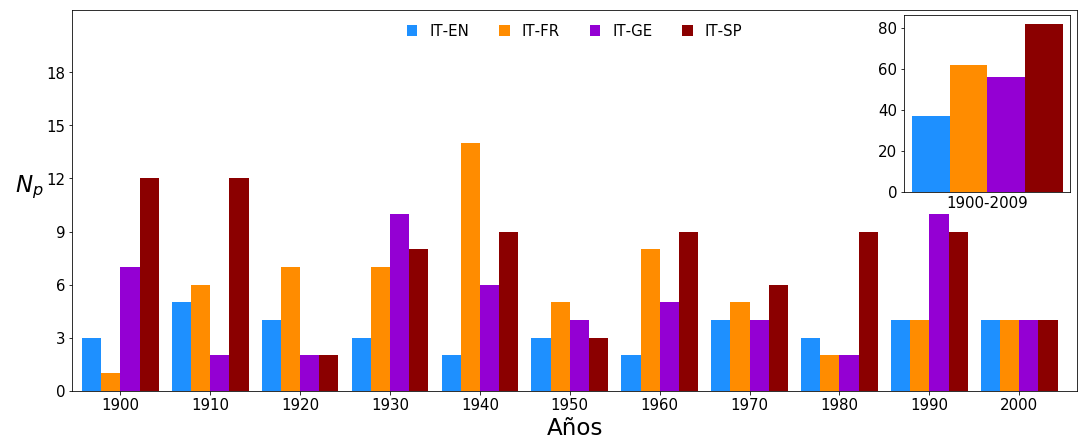
\includegraphics[scale=.33]{NC_IT.png}
	\caption{Palabras nuevas del italiano en los demás idiomas. Al provenir de la misma familia grecolatina, la fonética y la etimología son similares, por lo que  el español y el francés han adoptado la mayor cantidad de palabras provenientes del italiano.} 
	\label{fig.NC_IT}
\end{figure}



Entre todos los idiomas, las migraciones donde interviene el italiano son las mas homogéneas  entres la cantidades de palabras nuevas y palabras recibidas (al rededor de 20), apreciable en todas las posibles combinaciones de la figura~\ref{fig.NC_IT}.  

Unicamente con el ingles, el italiano ha sido exclusivamente un idioma  receptor, anteriormente en la página~\pageref{fig.NC_EN} se menciono a la segunda guerra mundial y al crecimiento económico de los Estados Unidos como causantes del dominio del inglés sobre el italiano. 

En los demás receptores,  el italiano fluctuá entre ser mayor portador o receptor de palabras,  con el alemán se dan dos periodo de crecimiento tras finalizar la primera guerra mundial y la guerra fria. Mientras que en las lenguas romances, la media de palabras  que el italiano aporta en cada década es de 6, con un mayor aumento entre 1930 y 1940.  


\subsubsection*{Italiano-Inglés}% {{{

A pesar de que en cada década existen términos nuevos en el inglés, sólo fue posible relacionar \textit{mussolini} (1935),  alusivo al político y militar Benito Mussolini, posiblemente el personaje italiano más relevante en la historia del siglo XX .

% }}}
\subsubsection*{Italiano-Francés}% {{{



En las migraciones sólo se asoció \textit{mussolini} (1935), la cual ya se había mencionado. Aunque en 1940 migraron la mayor cantidad de préstamos, ninguno de ellos ha tenido contexto con los sucesos de esa época. 

Tras revisar las listas de los préstamos nuevos con origen italiano  en los demás idiomas, Mussolini se encuentra en todas ellas, donde  el año de migración es siempre 1935.





% }}}
\subsubsection*{Italiano-Alemán}% {{{

En esta dirección existen relaciones con el contexto bélico,  \textit{regime} (1938), \textit{panzer} (1941), \textit{duce} (1942),  traducciones de régimen, blindado y líder.

%además de \textit{Mussolini} (1935). 



% }}}
\subsubsection*{Italiano-Español}% {{{

En el español, además de los términos de la guerra, se encontraron nombres de términos políticos y sociales que tuvieron un auge en el siglo pasado,  \textit{socialista} (1914), \textit{comunista} (1932), \textit{capitalismo} (1935), \textit{fascismo} (1937),  \textit{marxismo} (1963) y \textit{terrorismo} (1986). 

% }}}
% }}}
\subsection{Español}% {{{

\begin{figure} [h!] % {{{
	\centering
	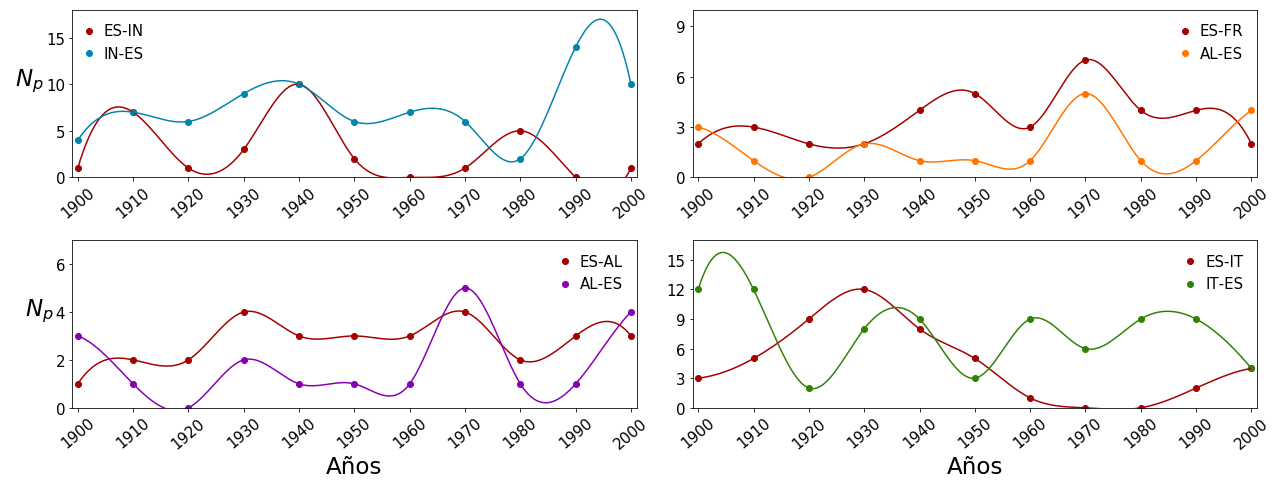
\includegraphics[scale=.33]{NC_SP.png}
	\caption{Palabras nuevas del español en los demás idiomas. El italiano es el idioma  que más palabras recibió del español, seguido del francés. En este sentido, las migraciones favorecen entre lenguas de la misma familia.}
	\label{fig.NC_SP}
\end{figure} % }}}

A partir de la figura~\ref{fig.NC_SP}, se aprecian dos similitudes entre las migraciones donde actuá el español.  La primera de ellas es entre el inglés y el italiano, en ambos la cantidad de palabras nuevas al tomar el español como origen o receptor) es similar  (entre cero y quince),  si se observan las migraciones que parten del español, las mayores ocurrencias suceden entre 1930 y 1950,  además existieron periodos sin alguna palabra nueva,  al rededor de 1960 en el ingles y entre 1970 y 1980 con el italiano. En estos idiomas, el español fue primordial mente un idioma receptor.

En la segunda relación con el francés y el alemán,  nuevamente la cantidad de palabras y el crecimiento del español en ambas lenguas es similar, al portar una media de cuatro palabras nuevas entre 1930 y el 1990 (con un incremento en ambos en 1970).




\subsubsection*{Español-Inglés}% {{{

Contrario a la tendencia en las migraciones anteriores, la guerra no es un campo semántico común en el contenido de los préstamos. La mayor parte de los términos son habituales en la medicina,  en 1943  aparecieron  \textit{virus} y \textit{anemia};  años antes en 1934 George Richards Minot, Parry Murphy y George Hoiyt Whipple, habían recibido el premio Nobel de medicina por su descubrimiento de la terapia de hígado para el tratamiento de anemias.   

Probablemente, las palabras virus y anemia ya existían en el inglés antes de 1943,  pero sólo hasta este año,  cobraron relevancia para ser parte de las cinco mil palabras más utilizadas. Esto ejemplifica que hay eventos (como un premio internacional) que retoman palabras cuyo periodo de uso  ha disminuido,  para volver a ser importantes y migrar a los demás idiomas.


\subsubsection*{Español-Francés}% {{{

El primer préstamo con contenido es \textit{panama} (1913), su importancia se debe a la inauguración del canal de Panamá en 1914, destaca que la palabra llegue al francés por ser el gobierno de Francia el que impulsó económicamente su construcción, aunque su conclusión y administración pasó a los Estados Unidos.  




% }}}
\subsubsection*{Español-Alemán}


Los préstamos son nuevamente términos médicos, además \textit{virus} y \textit{anemia} mencionados en las migraciones hacia el inglés, se encontró a \textit{lepra} (1901), anteriormente en 1874, Gerhard Armauer Hansen descubrió el bacilo de Leprae que origina la enfermedad.

%fue globalmente importante a partir de 1874,  ya que en ese año el científico noruego Gerhard Armauer Hansen descubrió el bacilo de Hansen Mycobacterium Leprae \cite{lepra} que origina la enfermedad. Por el carácter médico de la palabra, es probable que se hiciera más investigación sobre la enfermedad en diferentes idiomas, en este caso el alemán. 


% }}}
\subsubsection*{Español-Italiano}% {{{


Además de los términos medicos ya mencionados, en el italiano migraron de forma  exclusiva  \textit{virus} (1922), \textit{colesterina} (1928),  \textit{sintomatología} (1931), \textit{anestesia} (1932), \textit{vitamina} (1935), \textit{anemia} (1936), \textit{metabolismo} (1936),  \textit{gástrica} (1936)  y \textit{endovenosa} (1937).  

%El aparecer estas palabras en el español (dentro de las cinco mil más usadas)antes que en los demás,  sugiere que la medicina era un campo importante para los países de habla española, donde posiblemente se publicaron más libros de medicina en esta lengua. 






% }}}
% }}}
% }}}
\section{Resultados generales}% {{{



Tras las múltiples combinaciones entre idiomas, la relación habitual son palabras del campo semántico de la guerra, la mayor parte de ellas, surgieron en los diferentes receptores durante y después de la segunda guerra mundial. 

Cada idioma se muestra como un exportador de palabras de ciertos campos,  el inglés en economía, tecnología y política; el español en medicina; mientras el francés, el alemán y el italiano en la guerra.  

Las áreas mencionadas, no brindan una respuesta sobre que idioma ha sido más influyente, pero si en cuales campos un idioma ha influido más que los otros, siendo esta una forma alternativa de hablar de influencia en los idiomas.
 
Una manera diferente de estudiar a los préstamos nuevos, sería a través del tiempo que le toma a las palabras moverse de un idioma a otro, con ello, se pueden obtener la velocidad con la que migran y su adaptabilidad en las diferentes lenguas receptoras. Aunque estos resultados pueden ser complementarios, por el momento no se han tratado. 


%El inglés se presenta en las últimas dos décadas como el idioma común para transmitir información, exportando términos comunes en ámbitos como  la globalización y el desarrollo  de la tecnología.  Destaca el rol de los Estados Unidos como un país involucrado en los principales acontecimientos que originaron las migraciones, siendo usuales los apellidos de todos sus presidentes (posteriores a la segunda guerra mundial) en los demás idiomas. 

%Salvo el inglés que fue exportador en distintas áreas, los demás idiomas se caracterizaron por brindar palabras especificas,  el alemán por apellidos de personajes, el español por términos médicos, mientras que el francés y el italiano por la historia bélica y la religión. . 

 %Estos posibles resultados ayudarían a complementar la relación entre eventos, ya que en algunos eventos las palabras asociadas a él, migraron a los demás idiomas  en el mismo periodo, por ejemplo,  las palabras que migraron tras la revolución francesa (1789-1799) aparecieron en los diferentes receptores mientras ocurría el suceso y hasta veinte años después de él; así mismo,  los términos involucrados en la globalización  posterior a 1980 migraron en los años inmediatos a su invención.  Para tales complementos se necesitaría separar a los préstamos por áreas, lo cual no se hizo en este trabajo.  












% }}}



